% This is "sig-alternate.tex" V1.9 April 2009
% This file should be compiled with V2.4 of "sig-alternate.cls" April 2009
%
% This example file demonstrates the use of the 'sig-alternate.cls'
% V2.4 LaTeX2e document class file. It is for those submitting
% articles to ACM Conference Proceedings WHO DO NOT WISH TO
% STRICTLY ADHERE TO THE SIGS (PUBS-BOARD-ENDORSED) STYLE.
% The 'sig-alternate.cls' file will produce a similar-looking,
% albeit, 'tighter' paper resulting in, invariably, fewer pages.
%
% ----------------------------------------------------------------------------------------------------------------
% This .tex file (and associated .cls V2.4) produces:
%       1) The Permission Statement
%       2) The Conference (location) Info information
%       3) The Copyright Line with ACM data
%       4) NO page numbers
%
% as against the acm_proc_article-sp.cls file which
% DOES NOT produce 1) thru' 3) above.
%
% Using 'sig-alternate.cls' you have control, however, from within
% the source .tex file, over both the CopyrightYear
% (defaulted to 200X) and the ACM Copyright Data
% (defaulted to X-XXXXX-XX-X/XX/XX).
% e.g.
% \CopyrightYear{2007} will cause 2007 to appear in the copyright line.
% \crdata{0-12345-67-8/90/12} will cause 0-12345-67-8/90/12 to appear in the copyright line.
%
% ---------------------------------------------------------------------------------------------------------------
% This .tex source is an example which *does* use
% the .bib file (from which the .bbl file % is produced).
% REMEMBER HOWEVER: After having produced the .bbl file,
% and prior to final submission, you *NEED* to 'insert'
% your .bbl file into your source .tex file so as to provide
% ONE 'self-contained' source file.
%
% ================= IF YOU HAVE QUESTIONS =======================
% Questions regarding the SIGS styles, SIGS policies and
% procedures, Conferences etc. should be sent to
% Adrienne Griscti (griscti@acm.org)
%
% Technical questions _only_ to
% Gerald Murray (murray@hq.acm.org)
% ===============================================================
%
% For tracking purposes - this is V1.9 - April 2009

\documentclass{sig-alternate}
\usepackage{paralist}
\begin{document}
%
% --- Author Metadata here ---
\conferenceinfo{ANCS}{2011 Brooklyn, New York, USA}
%\CopyrightYear{2007} % Allows default copyright year (20XX) to be over-ridden - IF NEED BE.
%\crdata{0-12345-67-8/90/01}  % Allows default copyright data (0-89791-88-6/97/05) to be over-ridden - IF NEED BE.
% --- End of Author Metadata ---

\title{Efficient Implementation of Dynamic Protocol Stacks in Linux}
%
% You need the command \numberofauthors to handle the 'placement
% and alignment' of the authors beneath the title.
%
% For aesthetic reasons, we recommend 'three authors at a time'
% i.e. three 'name/affiliation blocks' be placed beneath the title.
%
% NOTE: You are NOT restricted in how many 'rows' of
% "name/affiliations" may appear. We just ask that you restrict
% the number of 'columns' to three.
%
% Because of the available 'opening page real-estate'
% we ask you to refrain from putting more than six authors
% (two rows with three columns) beneath the article title.
% More than six makes the first-page appear very cluttered indeed.
%
% Use the \alignauthor commands to handle the names
% and affiliations for an 'aesthetic maximum' of six authors.
% Add names, affiliations, addresses for
% the seventh etc. author(s) as the argument for the
% \additionalauthors command.
% These 'additional authors' will be output/set for you
% without further effort on your part as the last section in
% the body of your article BEFORE References or any Appendices.

\numberofauthors{3} %  in this sample file, there are a *total*
% of EIGHT authors. SIX appear on the 'first-page' (for formatting
% reasons) and the remaining two appear in the \additionalauthors section.
%
\author{
% You can go ahead and credit any number of authors here,
% e.g. one 'row of three' or two rows (consisting of one row of three
% and a second row of one, two or three).
%
% The command \alignauthor (no curly braces needed) should
% precede each author name, affiliation/snail-mail address and
% e-mail address. Additionally, tag each line of
% affiliation/address with \affaddr, and tag the
% e-mail address with \email.
%
% 1st. author
\alignauthor
Ariane Keller\\
       \affaddr{ETH Zurich, Switzerland}\\
       \email{ariane.keller@tik.ee.ethz.ch}
% 2nd. author
\alignauthor
Daniel Borkmann\\
        \affaddr{ETH Zurich, Switzerland}\\
        \affaddr{HTWK Leipzig, Germany}\\
        \email{borkmann@iogearbox.net}
% 3rd. author
\alignauthor 
Wolfgang M{\"u}hlbauer\\
       \affaddr{ETH Zurich, Switzerland}\\
       \email{muehlbauer@tik.ee.ethz.ch}
%\and  % use '\and' if you need 'another row' of author names
}
% There's nothing stopping you putting the seventh, eighth, etc.
% author on the opening page (as the 'third row') but we ask,
% for aesthetic reasons that you place these 'additional authors'
% in the \additional authors block, viz.
\date{30 July 2011}
% Just remember to make sure that the TOTAL number of authors
% is the number that will appear on the first page PLUS the
% number that will appear in the \additionalauthors section.

\maketitle
\begin{abstract}
TODO: rewrite abstract - beginning is copied from an old paper...
Future network architectures aim at solving the shortcomings of the traditional, static Internet architecture. In order to provide optimal service they have to adapt their functionality to different networking situations. This can be achieved by dividing the networking functionality into modular blocks and combining them as required at runtime.
In this paper we address the performance aspect of such architectures and we show that their performance is comparable with the performance of a standard Linux protocol stack.

\end{abstract}

% A category with the (minimum) three required fields
%\category{H.4}{Information Systems Applications}{Miscellaneous}
%A category including the fourth, optional field follows...
%\category{D.2.8}{Software Engineering}{Metrics}[complexity measures, performance measures]

%\terms{Theory}

%\keywords{ACM proceedings, \LaTeX, text tagging}

\section{Introduction}


Some references that might be useful: \cite{ANAJournal} (ANA) and \cite{click} (Click) and \cite{rba} (From protocol stack to protcol heap: role-based architecture) and \cite{Plutarch} (PLUTARCH:an arbument for network pluralism) and \cite{netgraph} (netgraph) and \cite{raj} (survey of next generation internet) and \cite{xKernel} (xKernel) and \cite{Zitterbart} (model for flexible high-performance communication subsystem). - should we explicitly say something on active networking or should we try to avoid it completely?


Placeholder: Lorem ipsum dolor sit amet, consectetur adipiscing elit. Pellentesque eu arcu ut est volutpat consequat sit amet dignissim enim. Lorem ipsum dolor sit amet, consectetur adipiscing elit. Nunc magna purus, vehicula sit amet fringilla ac, interdum ut dui. Ut in magna tortor, vitae dignissim lorem. Praesent condimentum eros aliquam mi pharetra egestas. Sed sem tortor, iaculis non ornare consequat, auctor eget velit. Nam nibh nibh, ullamcorper vitae gravida non, rhoncus vitae mi. Nunc vestibulum suscipit justo in laoreet. Praesent ac porta ante. Integer sem urna, pretium sed dignissim id, laoreet sit amet sem. Cras ac risus nec nibh tempor gravida. Integer ac ligula sed orci luctus condimentum at quis dui. Etiam dignissim dignissim tellus, et dapibus elit venenatis nec. Sed hendrerit imperdiet lacinia. Sed enim purus, mattis vel ullamcorper vel, malesuada vitae turpis. Pellentesque nec lacus tortor, eget scelerisque lectus. Suspendisse lectus mauris, tempor eget porttitor id, consectetur vel sem.

 Lorem ipsum dolor sit amet, consectetur adipiscing elit. Pellentesque eu arcu ut est volutpat consequat sit amet dignissim enim. Lorem ipsum dolor sit amet, consectetur adipiscing elit. Nunc magna purus, vehicula sit amet fringilla ac, interdum ut dui. Ut in magna tortor, vitae dignissim lorem. Praesent condimentum eros aliquam mi pharetra egestas. Sed sem tortor, iaculis non ornare consequat, auctor eget velit. Nam nibh nibh, ullamcorper vitae gravida non, rhoncus vitae mi. Nunc vestibulum suscipit justo in laoreet. Praesent ac porta ante. Integer sem urna, pretium sed dignissim id, laoreet sit amet sem. Cras ac risus nec nibh tempor gravida. Integer ac ligula sed orci luctus condimentum at quis dui. Etiam dignissim dignissim tellus, et dapibus elit venenatis nec. Sed hendrerit imperdiet lacinia. Sed enim purus, mattis vel ullamcorper vel, malesuada vitae turpis. Pellentesque nec lacus tortor, eget scelerisque lectus. Suspendisse lectus mauris, tempor eget porttitor id, consectetur vel sem. 
Praesent ac porta ante. Integer sem urna, pretium sed dignissim id, laoreet sit amet sem. Cras ac risus nec nibh tempor gravida. Integer ac ligula sed orci luctus condimentum at quis dui. Etiam dignissim dignissim tellus, et dapibus elit venenatis nec. Sed hendrerit imperdiet lacinia. Sed enim purus, mattis vel ullamcorper vel, malesuada vitae turpis. Pellentesque nec lacus tortor, eget scelerisque lectus. Suspendisse lectus mauris, tempor eget porttitor id, consectetur vel sem. 


\section{The Body of The Paper}

Description of the base architecture see Figure \ref{fig:architecture}.
\begin{compactitem}
\item Environment: kernel space - kernel XXX
\item Application Interface: socket API 
\item Hardware Interface: Vlink subsystem
\item Configuration: what can be configured?, Command line interface 
\item Internals: state Management, Functional block notifier 
\end{compactitem}

\begin{figure}
\centering
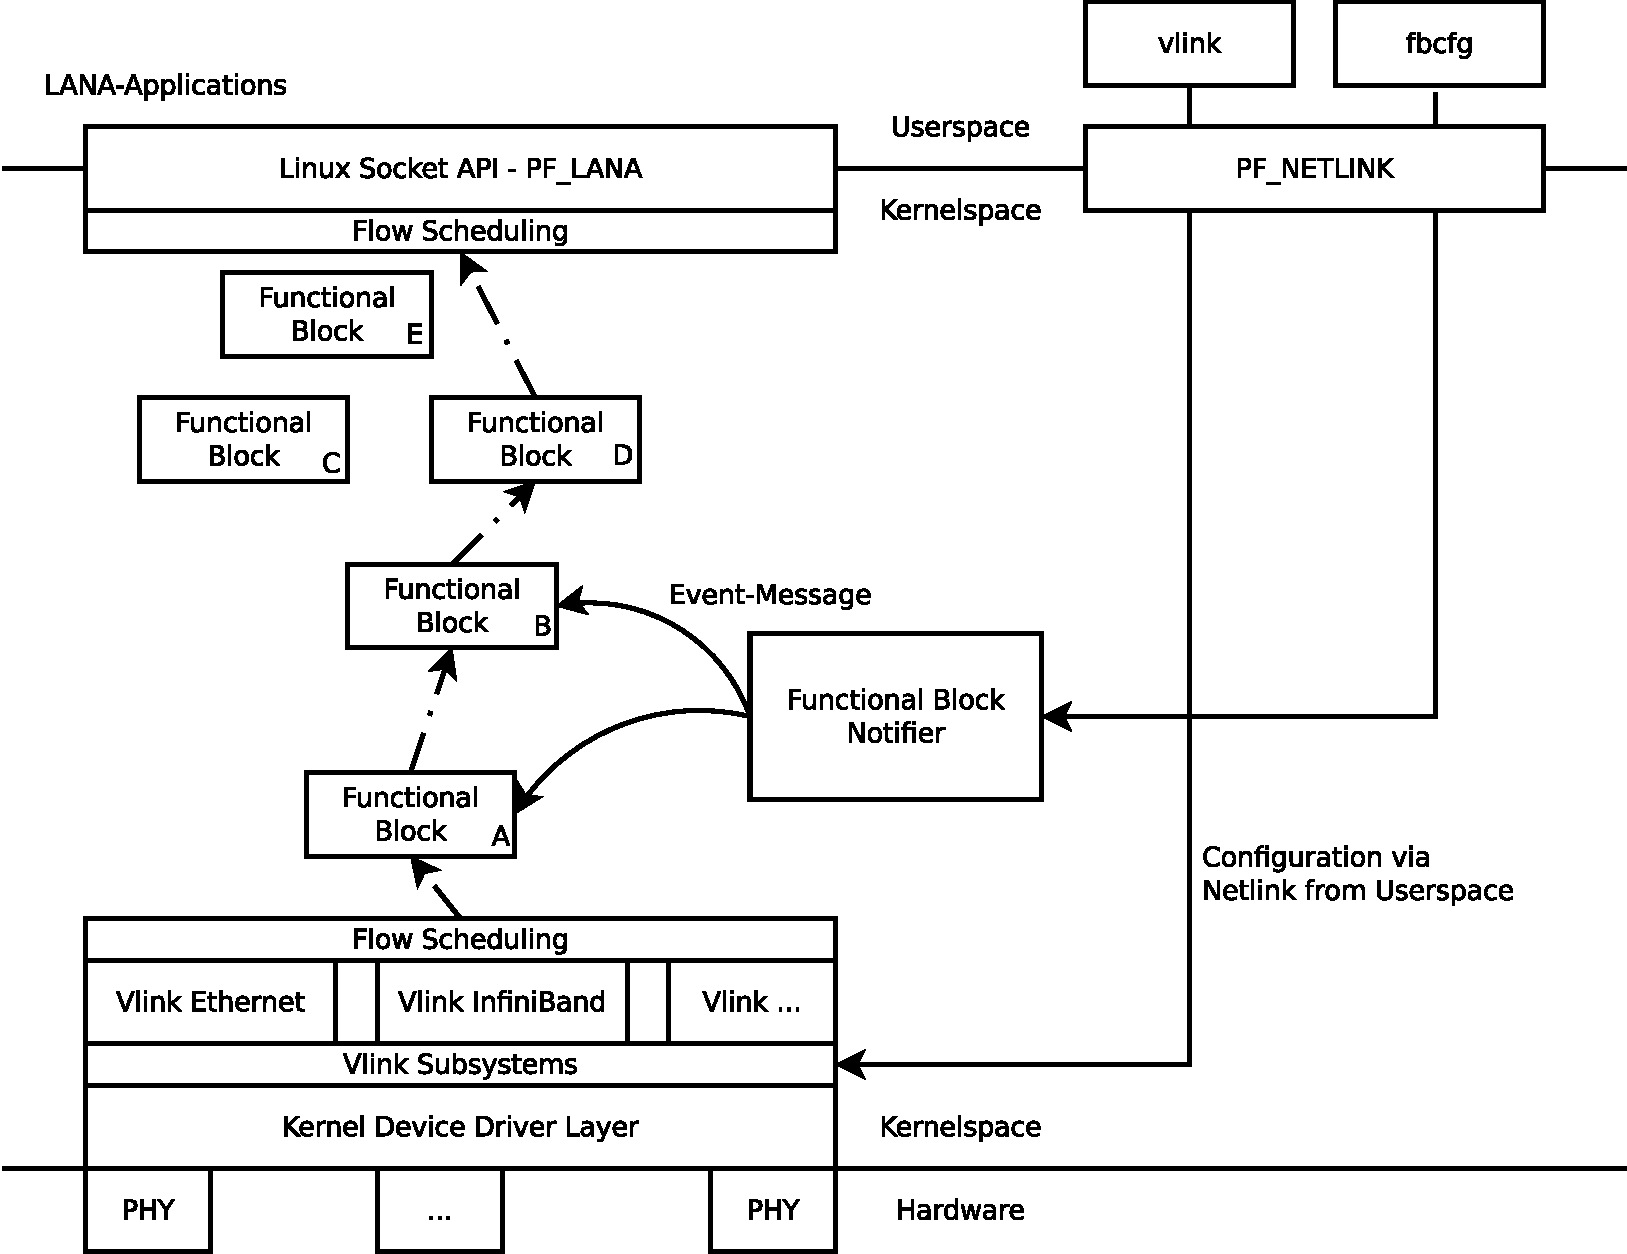
\includegraphics[width=0.47\textwidth]{figures/architecture.pdf}
%\epsfig{file=fly.eps}
\caption{Lana architecture}
\label{fig:architecture}
\end{figure}

%\begin{figure}
%\centering
%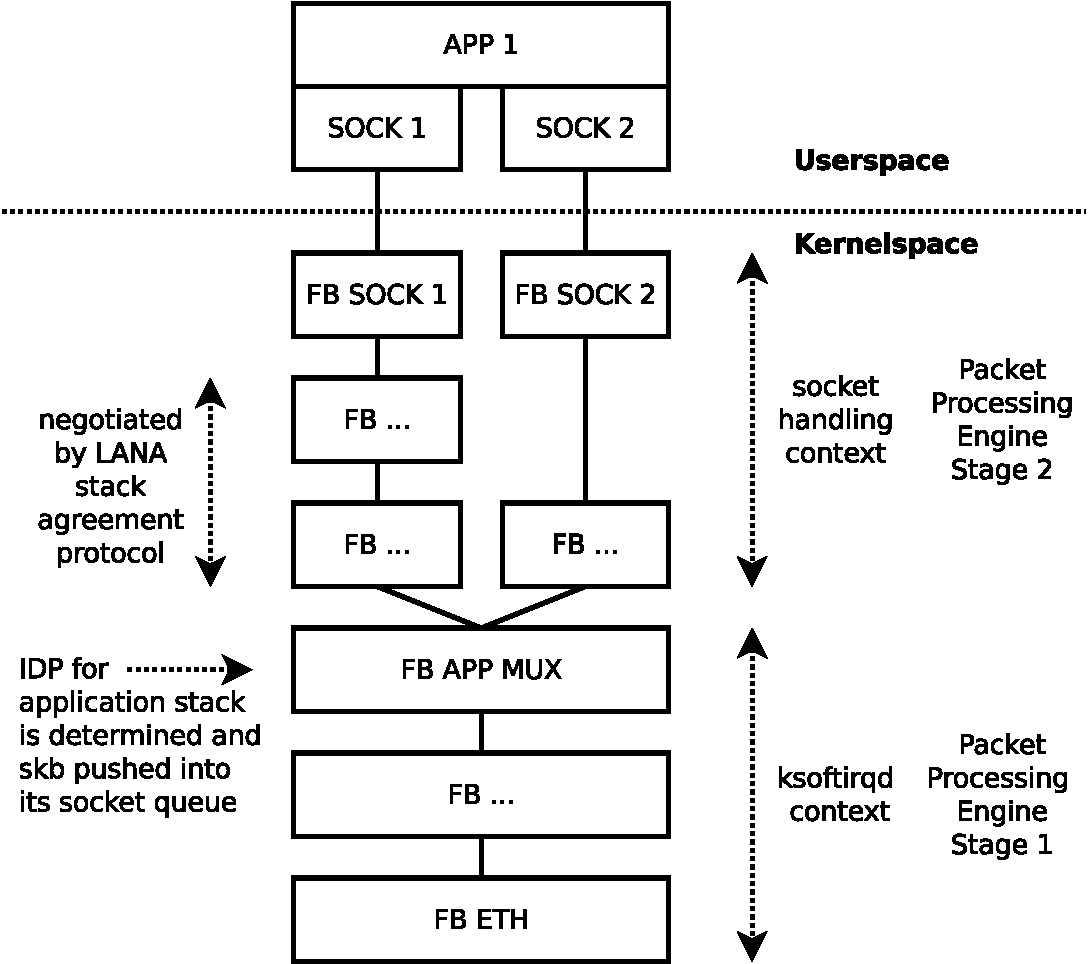
\includegraphics[width=0.4\textwidth]{figures/stack.pdf}
%\caption{Lana protocol stack showing in which contex which functionality is implemented}
%\label{fig:stack}
%\end{figure}

\subsection{Configuration Interface}
The protocol stack can be configured from user space with the help of a command line tool. The most important commands are summarized below.
\begin{compactitem}
\item \texttt{add}, \texttt{rm}: Adds (removes) a functional block from the list of available functional blocks in the kernel. 
\item \texttt{set}: sets properties of a functional block with a \texttt{key=value} semantic
\item \texttt{bind}, \texttt{unbind}: Binds (unbinds) a functional block to another in order to be able to send messages to it. 
\item \texttt{replace}: Replaces one functional block with another functional block. The connections between the blocks are maintained. Private data can either be transferred to the new block or dropped.
\item \texttt{subscribe}, \texttt{unsubscribe}: Subscribes (Unsubscribes) one functional block to receive control messages from another functional block.
\end{compactitem}

\subsection{Improving the Performance}
During the implementation of our framework we have evaluated different possibilities for the integration of our packet processing engine with the Linux kernel. We think the insights gained are interesting for other researcher that have to do fundamental changes on the Linux protocol stack and hence, we summarize them here. 
Our goal was to be able to process as many \textit{minimum sized Ethernet frames} as the Linux kernel is able to process. In order to compare the performance of the Linux Kernel and the performance of our engine we have dropped all packets in the Linux Kernel protocol stack as soon as they were arrived (TODO: where exactly?). In our system the packets were processed by the fb\_eth functional block followed by two fb\_dummy functional blocks that were simply forwarding the packets. We can distinguish the following three approaches:
\begin{compactitem}
\item On each CPU there exists one high priority thread that is responsible for processing LANA packets. This approach leads to a starvation of the interrupt handler (ksoftirqd) and hence the maximal achieved packet rate is only about half as what is achieved by the protocol stack of the Linux kernel. Also changing the priority of the LANA thread to normal only slightly increases the throughput.
\item Instead of relying completely on the Scheduler of the Linux Kernel we control preemption and scheduling explicitly. This approach still exhibits scheduling overhead, but it increases the performance to about two thirds of the performance of the Linux Kernel. 
\item Instead of executing the LANA functions in a dedicated thread they are executed directly in the ksoftirqd function. With this approach approximately $95\%$ of the performance of the Linux kernel is achieved.
\end{compactitem}
The corresponding numbers are listed in Table \ref{tab:performance}.

\begin{table}[htb]
\begin{tabular}{ l l }
mechanism & performance\\
\hline
dedicated kernel thread (high priority) & 700000\\
dedicated kernel thread (normal priority) & 750000\\
dedicated kernel thread (controlled scheduling) & 900000\\
execution in ksoftirqd & 130000\\
Linux kernel stack & 138000\\
\end{tabular}
\caption{Performance evaluation (pps) of different approaches to receiving packets in the Linux kernel. The packets are 64 Bytes long. The evaluation was done on a TODO: CPU/RAM/NETWORKCARD/KERNEL}
\label{tab:performance}
\end{table}	

\subsection{Software Available}
The current sofware is available under the GNU General Public License from \cite{lana}. In addition to the framework it also includes four functional blocks: Ethernet, Berkeley Packet Filter, Tee (duplicate a packet), and Forward (an empty Block that just forwards the packets to another block). The framework does not need any patching of the Linux kernel but needs a new, 2.6.X kernel.

\section{Conclusions and Future Work}
We have shown that it is possible to implement a flexible protocol stack that has a similar performance than the default protocol stack in the Linux kernel. This allows for the easy inclusion of new, still to be developed protocols and for the change of the protocol stack at runtime to include for example compression or encryption as the networking conditions change. 

In the short term we will compare the performance of real scenarios implemented in our system with the performance of an implementation in other systems (for example default Linux protocol stack or the Click router). In the midterm we will develop a mechanism that automatically sets up a protocol stack for an Application whereby the Application can specify some characteristics the communication channel should have, but not exactly how this has to be achieved. For example the application could require a "reliable communication channel" and a controller would choose between different protocols that provide reliability (e.g., one for wired communication, one for wireless communication, one for wireless, multi-hop communication). The setup of the protocol stack will have to be negotiated between the source and destination node. The end goal will be to have a networked system that requires less configuration as compared to todays networks and that is able to adapt itself to changing network conditions.   


%\end{document}  % This is where a 'short' article might terminate

%ACKNOWLEDGMENTS are optional
\section{Acknowledgments}
The research leading to these results has received funding from the European Union Seventh Framework Programme under grant agreement $n^o 257906$.
%
% The following two commands are all you need in the
% initial runs of your .tex file to
% produce the bibliography for the citations in your paper.
\bibliographystyle{abbrv}
\bibliography{epics}  % sigproc.bib is the name of the Bibliography in this case
% You must have a proper ".bib" file
%  and remember to run:
% latex bibtex latex latex
% to resolve all references
%
% ACM needs 'a single self-contained file'!
%
%APPENDICES are optional
%\balancecolumns
\end{document}
